\section*{Component specific Types}

\begin{table}[!htb] 
    \label{api:selectComponentTypes}
    \footnotesize
    \setlength\extrarowheight{4pt}
    \begin{tabular}{ p{5cm} p{8cm}}
        \toprule[1.2pt]
        \textbf{Type}    & \textbf{Description} \\
        \midrule    
        SimpleOption & \{ label: String?, value: String \}    \\
        OptionData   & \{ String | SimpleOption \}        \\
        OptionsTable & Array$<$Array$<$OptionData$>>$       \\
        Callback     & (...String) => Array$<$OptionData$>$ \\
        \bottomrule[1.2pt]
    \end{tabular}
\end{table}

\vspace*{12pt}
The \codestyle{SelectAttributes} object contains the following properties: 

\begin{table}[!htb] 
    \label{api:selectComponentSelectAttributes}
    \footnotesize
    \setlength\extrarowheight{4pt}
    \begin{tabular}{ p{4cm} p{3cm} p{6cm} }
        \toprule[1.2pt]
        \textbf{Property}             & \textbf{Type} & \textbf{Description} \\
        \midrule
        label                         & String        & Content of the Label for the input. \\
        name                          & String        & Name of the input that is sent with the form. \\
        isRequired                    & Boolean       & Defines if the selection of an option is required to send the form. \\
        isDisabled                    & Boolean       & Defines if the value can be changedand if the interaction work. \\
        isCursorPositionWithSelection & Boolean       & Defines if the cursor position is linked with the selection. 
                                                        If true: the keyboard interaction directly changes the selection. \\
        \bottomrule[1.2pt]
    \end{tabular}
\end{table}


% ---------
\clearpage
\section*{Components}

\vspace*{6pt}
\subsection*{SelectComponentByCallbacks}

\vspace*{6pt}
Creates an input component with the functionality: selecting an option in a given list. 

\vspace*{18pt}
\noindent
\textbf{Returns}: \codestyle{SelectComponent}

\begin{table}[!htb] 
    \label{api:selectComponentByCallbacksReturn}
    \footnotesize
    \setlength\extrarowheight{4pt}
    \begin{tabular}{ p{3.5cm} p{3.5cm} p{6cm} }
        \toprule[1.2pt]
        \textbf{Function}     & \textbf{Type}        & \textbf{Description} \\
        \midrule
        getSelectController() & SelectController & Provides the whole functionality of the select component. \\
        getComponentView()    & HTMLDivElement   & Provides the whole view with the select element and the label. \\
        getLabelElement()     & HTMLLabelElemen  & Provides the label element from the whole view. \\
        \bottomrule[1.2pt]
    \end{tabular}
\end{table}

\vspace*{6pt}
\noindent
\textbf{Parameters}

\begin{table}[!htb] 
    \label{api:selectComponentByCallbacksParameter}
    \footnotesize
    \setlength\extrarowheight{4pt}
    \begin{tabular}{ p{3.5cm} p{3.5cm} p{6cm} }
        \toprule[1.2pt]
        \textbf{Name}    & \textbf{Type}    & \textbf{Description} \\
        \midrule
        selectAttributes & SelectAttributes & Defines properties to customize the select component. \\
        serviceCallbacks & Array<Callback>  & Lists the Callback functions that provide the data for the options. 
                                              The number of callbacks in the array define the number of colums in the component. 
                                              The most right or biggest indexed callback in the array contains the value providing function. 
                                              The order is defined as in the view: from most general categry to specific value. 
                                              As parameter the callbacks take the string of the parent category of the current column. \\
        \bottomrule[1.2pt]
    \end{tabular}
\end{table}

\vspace*{6pt}
\noindent
\textbf{Example}

\begin{lstlisting}[style = htmlcssjs, label = api:selectComponentCbExample]
const getYearsByDecade = (...decades) => {
    const decadeStarts = decades.map(decade => decade.slice(0, 3));
    const data         = [...Array(70).keys()].map((e) => e + 1940 + "");
    return data.filter((e) => decadeStarts.length === 0 || decadeStarts.includes(e.slice(0, 3)));
};
const decades = [...Array(7).keys()].map((e) => e * 10 + 1940 + "'s");

const selectAttribute = { name : "year", label: "Year" };
const columnServiceCb = [ () => decades, getYearsByDecade ];
const selectComponent = SelectComponentByCallbacks(
    selectAttribute,
    columnServiceCb
);

const componentYear   = document.getElementById("componentContainer");
componentYear.append(selectComponent.getComponentView());
\end{lstlisting}
    
\begin{figure}[!htb]
    \centering
    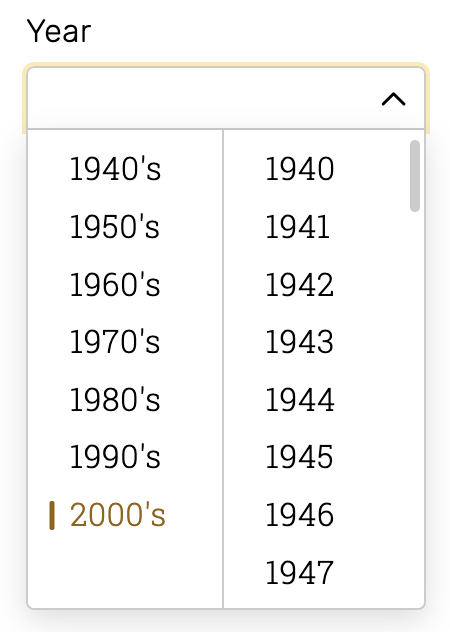
\includegraphics[width=80mm]{newComponent/opened.2col.png}
    \caption*{\centering Beispiel \codestyle{SelectComponentByCallbacks}}
    \label{api:selectComponentCbImg}
\end{figure}


% ---------
\clearpage
\subsection*{SelectComponentByTableValues}

\vspace*{6pt}
Creates an input component with the functionality: selecting an option in a given list. 

\vspace*{18pt}
\noindent
\textbf{Returns}: \codestyle{SelectComponent}

\begin{table}[!htb] 
    \label{api:selectComponentByTableValuesReturn}
    \footnotesize
    \setlength\extrarowheight{4pt}
    \begin{tabular}{ p{3.5cm} p{3.5cm} p{6cm} }
        \toprule[1.2pt]
        \textbf{Function}     & \textbf{Type}    & \textbf{Description} \\
        \midrule
        getSelectController() & SelectController & Provides the whole functionality of the select component. \\
        getComponentView()    & HTMLDivElement   & Provides the whole view with the select element and the label. \\
        getLabelElement()     & HTMLLabelElemen  & Provides the label element from the whole view. \\
        \bottomrule[1.2pt]
    \end{tabular}
\end{table}

\vspace*{6pt}
\noindent
\textbf{Parameters}

\begin{table}[!htb] 
    \label{api:selectComponentByTableValuesParameter}
    \footnotesize
    \setlength\extrarowheight{4pt}
    \begin{tabular}{ p{4.5cm} p{3cm} p{5.5cm} }
        \toprule[1.2pt]
        \textbf{Name}                 & \textbf{Type}    & \textbf{Description} \\
        \midrule
        selectAttributes              & SelectAttributes & Defines properties to customize the select component. \\
        optionsTable                  & OptionsTable     & Lists the options with all the categories denormalized. 
                                                           Each Entry in the outer array contains one OptionData per column. 
                                                           If a value has multiple categories in the same column, it needs multiple entries. 
                                                           If a value has no categry in a column `null` can be placed in that place. 
                                                           Every entry shuold have the same length and defines the options from most general category to value. 
                                                           The shortest entry array defines the number of columns. 
                                                           The category columns will use the distinct OptionData as options. \\
        sortColumnOptionsAlphabetical & Boolean          & Defines if the options of each column are sorted alphabetically. 
                                                           The sorting will be applied to every column or none of them. \\
        \bottomrule[1.2pt]
    \end{tabular}
\end{table}

\vspace*{6pt}
\noindent
\textbf{Example}

\begin{lstlisting}[style = htmlcssjs, label = api:selectComponentTvExample]
const tableOptions    = [ 
    [ "1940's", 1940 ], 
    [ "1940's", 1941 ], 
    [ "1940's", 1942 ], 
    [ "1940's", 1943 ], 
    /* ... */
    [ "1950's", 1958 ], 
    [ "1950's", 1959 ], 
    [ "1960's", 1960 ], 
    [ "1960's", 1961 ], 
    /* ... */
    [ "2000's", 2007 ], 
    [ "2000's", 2008 ], 
    [ "2000's", 2009 ], 
];
const selectAttribute = { name : "year", label: "Year" };
const selectComponent = SelectComponentByTableValues(
    selectAttribute,
    tableOptions
);

const componentYear   = document.getElementById("componentContainer");
componentYear.append(selectComponent.getComponentView());
\end{lstlisting}
    
\begin{figure}[!htb]
    \centering
    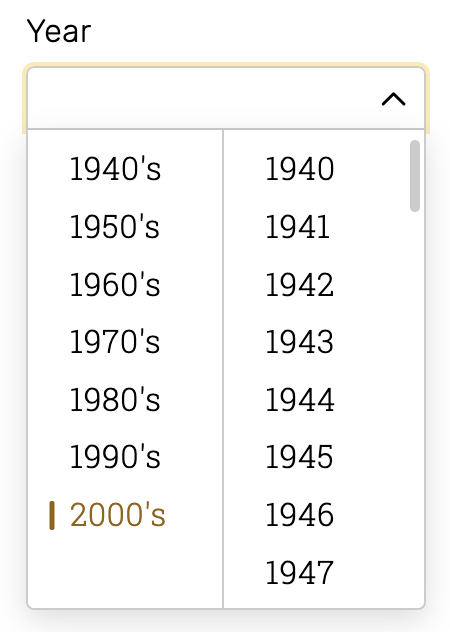
\includegraphics[width=80mm]{newComponent/opened.2col.png}
    \caption*{\centering Beispiel \codestyle{SelectComponentByTableValues}}
    \label{api:selectComponentTvImg}
\end{figure}


% ---------
\clearpage
\subsection*{ColumnOptionsComponent}

\vspace*{6pt}
Creates a column view of a given list of options. 

\vspace*{18pt}
\noindent
\textbf{Returns}: \codestyle{ColumnOptionsComponent}

\begin{table}[!htb] 
    \label{api:columnOptionsComponentReturn}
    \footnotesize
    \setlength\extrarowheight{4pt}
    \begin{tabular}{ p{5cm} p{3cm} p{5cm} }
        \toprule[1.2pt]
        \textbf{Function}                   & \textbf{Type}  & \textbf{Description} \\
        \midrule
        getOptions()                        & Array<Option>  & Lists all options contained in the column. 
                                                               The order is the one from adding the options. \\
        addOptions(Array<Option>)           & void           & Adds all passed options to the end of the column. 
                                                               If an option is alreayd contained it is ignored while adding. 
                                                               Options count as same if the label and the value are same. \\
        delOptions(Array<Option>)           & void           & Removes all passed options from the column. 
                                                               If an option is not contained the code just continues. 
                                                               Options count as same if the label and the value are same. \\
        clearOptions()                      & void           & Removes all options from the column. \\
        getSelectedOption()                 & Option         & Read the selected option. \\
        setSelectedOption(Option)           & void           & Changes the selected option to the passed option. 
                                                               Only one option can be selected in the column component. \\
        clearSelectedOption()               & void           & Resets the selection to nothing selected. \\
        \tbbr{
            onOptionSelected( \\
                \ \ \ Consumer<Option>
            )}                              & void           & Adds a listener to the change of the option selection observable. \\
        isSelectedOptionDisabled()          & Boolean        & Checks if the selected option is disabled to be changed. \\
        setSelectedOptionDisabled(bool)     & void           & Changes the possibility to change the selection. 
                                                               Sets the disabled to the passed value. 
                                                               If true the selection cannot be changed. \\
        \tbbr{
            onSelectedOptionDisabledChanged( \\
                \ \ \ Consumer<Option>
            )}                              & void           & Adds a listener to the change of the disable observable. \\
        getColumnView()                     & HTMLDivElement & Provides the whole column component. 
                                                               It is not linked to an input field. \\
        \bottomrule[1.2pt]
    \end{tabular}
\end{table}

\vspace*{6pt}
\noindent
\textbf{Parameters}

\begin{table}[!htb] 
    \label{api:columnOptionsComponentParameter}
    \footnotesize
    \setlength\extrarowheight{4pt}
    \begin{tabular}{ p{3.2cm} p{4.2cm} p{5.6cm} }
        \toprule[1.2pt]
        \textbf{Name}            & \textbf{Type}            & \textbf{Description} \\
        \midrule
        cursorPositionController & SelectedOptionController & Controller for the current cursor position. 
                                                              The cursor position is used as indicator at which option the keyboard is currently at. \\
        columnNumber             & Number?                  & Optional position of index of the column. 
                                                              It is used to identify the column in a select component. \\
        \bottomrule[1.2pt]
    \end{tabular}
\end{table}

\vspace*{6pt}
\noindent
\textbf{Example}

\begin{lstlisting}[style = htmlcssjs, label = api:columnOptionsComponentExample]
const cursorPos = SelectedOptionController();
const component = ColumnOptionsComponent(cursorPos);
document.getElementById("componentContainer").append(component.getColumnView());

const selectedOption = CategoryOption("selected");
const options = [ 
    selectedOption,
    CategoryOption("cat 1"),
    CategoryOption("cat 2"),
    CategoryOption("cat 3") 
];

component.addOptions(options);
component.setSelectedOption(selectedOption);

document.querySelector("head style").textContent += pageCss;
\end{lstlisting}

\begin{figure}[!htb]
    \centering
    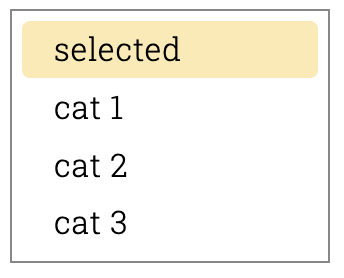
\includegraphics[width=50mm]{columnOptionsExample.png}
    \caption*{\centering Beispiel \codestyle{Column\-Options\-Component}}
    \label{api:columnOptionsComponentImg}
\end{figure}


% ---------
\clearpage
\section*{Controller}

\vspace*{6pt}
\subsection*{SelectController}

\vspace*{6pt}
Provides the functionality to manage a select input component. 

\vspace*{18pt}
\noindent
\textbf{Returns}: \codestyle{SelectComponent}

\begin{table}[!htb] 
    \label{api:selectControllerReturn}
    \footnotesize
    \setlength\extrarowheight{4pt}
    \begin{tabular}{ p{5cm} p{3cm} p{5cm} }
        \toprule[1.2pt]
        \textbf{Function}                    & \textbf{Type}          & \textbf{Description} \\
        \midrule
        getId()                              & String                 & Provides a unique id for each component. \\
        getNumberOfColumns()                 & Number                 & Provides the fixed number of columns to show in the ui. \\
        getInputController()                 & SimpleInputController  & Provides the functionality of the text input hidden behind the component. 
                                                                        This input will send the data in the from. \\
        isCursorPositionWithSelection()      & Boolean                & Checks if the keyboard interaction also changes the selection. 
                                                                        If false the cursor position for the keyboard acts like the highlight for the mouse. \\
        isRequired()                         & Boolean                & Checks if an option has to be chosen in a form. \\
        setRequired(Boolean)                 & void                   & Changes the requirement of the select input to the passed value. \\
        \tbbr{
            onRequiredChanged( \\
                \ \ \ Consumer<Option>
            )}                               & void                   & Adds a listener to the change of the requirement. \\
        isDisabled()                         & Boolean                & Checks if the option of the select input can be changed.  \\
        setDisabled(Boolean)                 & void                   &  \\
        \tbbr{
            onDisabledChanged( \\
                \ \ \ Consumer<Option>
            )}                               & void                   & Adds a listener to the change of possibility to fill the input. \\
        isOptionsVisible()                   & Boolean                & Checks if the options container is visible. 
                                                                        It contains all the category and value options. 
                                                                        In a default select this would be the not visible part of the component in the initial state. \\
        setOptionsVisibility(Boolean)        & void                   & Change the visibility of the options container to the passed value. \\
        \tbbr{
            onOptionsVisibilityChange( \\
                \ \ \ Consumer<Option>
            )}                               & void                   & Adds a listener to the change of the visibility of the options container. 
                                                                        It contains all the category and value options. 
                                                                        In a default select this would be the not visible part of the component in the initial state. \\
        isSelectedOptionVisible()            & Boolean                & Checks if the selected option container is visible. 
                                                                        It contains only the selected option and maybe some action buttons. 
                                                                        In a default select this would be the always visible part of the component. \\
        setSelectedOptionVisibility(Boolean) & void                   & Change the visibility of the selected option container to the passed value. \\
        \tbbr{
            onSelectedOptionVisibilityChange( \\
                \ \ \ Consumer<Option>
            )}                               & void                   & Adds a listener to the change of the visibility of the selected option container. 
                                                                        It contains only the selected option and maybe some action buttons. 
                                                                        In a default select this would be the always visible part of the component. \\
        \bottomrule[0.5pt]
    \end{tabular}
\end{table}

\clearpage
\begin{table}[!htb] 
    \label{api:selectControllerReturn2}
    \scriptsize
    \setlength\extrarowheight{4pt}
    \begin{tabular}{ p{5cm} p{2.3cm} p{5.7cm} }
        \toprule[0.5pt]
        \textbf{Function}                    & \textbf{Type}          & \textbf{Description} \\
        \midrule    
        getCursorPosition()                  & Option                 & Provides the option the keyboard cursor is currently at. \\
        setCursorPosition(Option)            & void                   & Changes the cursor position of the keyboard to the passed option. 
                                                                        The cursor position can only  contain one option per component. \\
        clearCursorPosition()                & void                   & Reset the keyboard cursor to no option. \\
        \tbbr{
            onCursorPositionChanged( \\
                \ \ \ Consumer<Option>
            )}                               & void                   & Adds a listener to the change of the cursor position. \\
        getSelectedValueOption()             & Option                 & Provides the selected value option of the select input. 
                                                                        This is the option that is sent in a form. \\
        setSelectedValueOption(Option)       & void                   & Changes the selected value option to the passed option. 
                                                                        There can only be one option selected.  \\
        clearSelectedValueOption()           & void                   & Reset the selected value option to no option.  \\
        getSelectedOptionOfColumns(Number)   & Option                 & Provides the selected option of the passed column. 
                                                                        The column 0 contains the same value as in `getSelectedValueOption()` is provided. 
                                                                        The other columns contain the selected category of the passed column. \\
        getColumnOptionsComponent(Number)    & \raggedright Column\-
                                               Options\-Component     & Provides the column options compontent of the passed column with the view and functionality. 
                                                                        The column 0 provides the value option column component. 
                                                                        The other columns provide the category option columns of the passed column. \\
        \bottomrule[1.2pt]
    \end{tabular}
\end{table}

\vspace*{6pt}
\noindent
\textbf{Parameters}

\begin{table}[!htb] 
    \label{api:selectControllerParameter}
    \footnotesize
    \setlength\extrarowheight{4pt}
    \begin{tabular}{ p{3.2cm} p{3cm} p{6.8cm} }
        \toprule[1.2pt]
        \textbf{Name}    & \textbf{Type}       & \textbf{Description} \\
        \midrule
        selectAttributes & SelectAttributes & Defines properties to customize the select component. \\
        numberOfColumns  & Number           & Defines the number of columns in the options container. \\
        \bottomrule[1.2pt]
    \end{tabular}
\end{table}

\vspace*{6pt}
\noindent
\textbf{Example}

\begin{lstlisting}[style = htmlcssjs, label = api:selectControllerExample]
const decades = [
    ValueOption("1990's"),
    ValueOption("2000's"),
    ValueOption("2010's"),
    ValueOption("2020's")
];
const currentYear = CategoryOption("2024");
const years = [
    CategoryOption("1990"),
    CategoryOption("1991"),
    /* ... */
    CategoryOption("2009"),
    CategoryOption("2010"),
    /* ... */
    CategoryOption("2023"),
    currentYear
];
const selectAttributes = { 
    name : "year", 
    label: "Year", 
    isRequired: true 
};
const selectController = SelectController(selectAttributes, 2);

selectController.getColumnOptionsComponent(1).onOptionSelected(
    newDecade => {
        selectController.getColumnOptionsComponent(0).clearOptions();
        selectController.getColumnOptionsComponent(0).addOptions(
            years.filter(year => year.getLabel().startsWith(
                newDecade.getLabel().slice(0, 2)))
        );
});
selectController.getColumnOptionsComponent(0).onOptionSelected(
    newDecade => alert("You chose the year: " + newDecade.getLabel()));

selectController.getColumnOptionsComponent(1).addOptions(descades);
selectController.getColumnOptionsComponent(0).addOptions(years);

selectController.getColumnOptionsComponent(0)
                .setSelectedOption(currentYear);
\end{lstlisting}